\newpage

\newpage
\newpage
\newpage

\section{Introduction to Static Single Assignment}

Many dataflow analyses need to find the use-sites of each defined variable or the definition-sites of each variable used in an expression. The \textit{def-use chain} is a data structure that makes this efficient: for each statement in the flow graph, the compiler can keep a list of pointers to all the use sites of variables defined there, and a list of pointers to all definition sites of the variables used there. An improvement on the idea of def-use chains is static single-assignment form, or SSA form, an intermediate representation in which each variable has only one definition in the program text. SSA is very useful for many optimizations such as Loop-Invariant Code Motion and Copy Propagation.

% \subsection{Motivation}

% \begin{itemize}
%     \item The values in reused locations may be provably independent.
%     \item It would be nice if we could traverse directly between related uses and def's
% \end{itemize}

\subsection{Definition-Use and Use-Definition Chains}


\begin{definition}{Use-Definition (UD) Chains}
For a given definition of a variable X, what are all of its uses?

\end{definition}



\begin{definition}{Definition-Use (DU) Chains}
For a given use of a variable X, what are all of the reaching definitions of X?

\end{definition}



Unfortunately, it is expensive to use UD and DU chains, because if we have N defs, and M uses, the space complexity is O(NM). An example is in \ref{fig:p38}


\begin{figure}[htb]
    \centering
    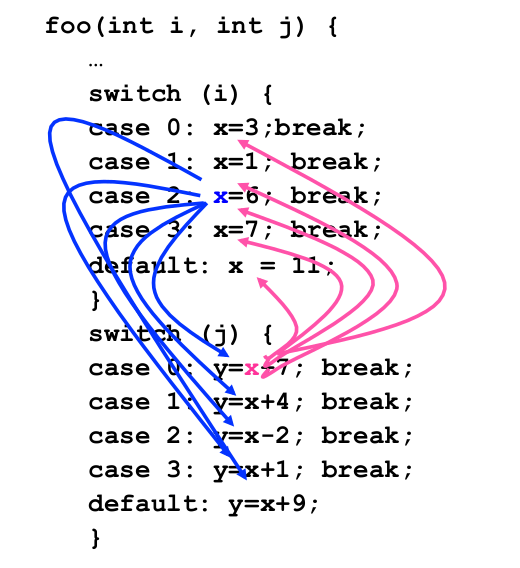
\includegraphics[width=0.3\textwidth]{p38.png}
    \caption{If a variable has N uses and M definitions (which occupy about N + M instructions in a program), it takes space (and time) proportional to N · M to represent def-use chains – a quadratic blowup.}
    \label{fig:p38}
\end{figure}


\subsection{Static Single Assignment(SSA)}

\begin{definition}{Static Single Assignment }
    Static Single Assignment is an IR where every variable is assigned a value at most once in the program text.
\end{definition}








\begin{definition}{the $\Phi$ function}

     $\Phi$ merges multiple definitions along multiple control paths into a single definition.

     At a basic block with p predecessors, there are p arguments to the $\Phi$ functions.

     $$ x_{\text {new }} \leftarrow \Phi\left(\mathbf{x}_1, \mathbf{x}_1, \mathbf{x}_1, \ldots, \mathbf{x}_{\mathrm{p}}\right)
     $$
\end{definition}

\subsubsection{Why SSA is useful?}

\textbf{ \large \textit{Useful for Dataflow Analysis}} Dataflow analysis and optimization algorithms can be made simpler when each variable has only one definition.

\textbf{ \large \textit{Less space and time complexity}} If a variable has N uses and M definitions (which occupy about N + M instructions in a program), it takes space (and time) proportional to N · M to represent def-use chains – a quadratic blowup. For almost all realistic programs, the size of the SSA form is linear in the size of the original program.


\textbf{ \large \textit{Simplify some algorithms}} Uses and defs of variables in SSA form relate in a useful way to the dominator structure of the control-flow graph, which simplifies algorithms such as interference-graph construction.


\textbf{ \large \textit{Eliminate needless relationship}} Unrelated uses of the same variable in the source program become different variables in SSA form, eliminating needless relationships shown in \ref{exp:1}.

\begin{lstlisting}[label={exp:1},caption={An example}]

for i <- 1 to N do A[i] <- 0
for i <- 1 to M do s <- s + B[i]

\end{lstlisting}


\subsection{How to represent SSA?}

In straight-line code, such as within a basic block, it is easy to see that each instruction can define a fresh new variable instead of redefining an old one shown in \ref{fig:p42-43}


\begin{figure}[htb]
     \centering
     \begin{subfigure}{0.2\textwidth}
     \centering
         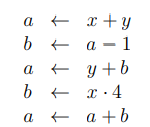
\includegraphics[width=\textwidth]{p42.png}
         \caption{A straight-line program.}
         \label{fig:p42}
     \end{subfigure}
     \begin{subfigure}{0.25\textwidth}
     \centering
         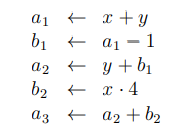
\includegraphics[width=\textwidth]{p43.png}
         \caption{The program in single-assignment form.}
         \label{fig:p43}
     \end{subfigure}
        \caption{SSA for straight-line code}
        \label{fig:p42-43}
\end{figure}


But when two control-flow paths merge together, it is not obvious how to have only one assignment for each variable. To solve this problem we introduce a notational fiction, called a $\Phi$ function. Figure \ref{fig:p44} shows that we can combine a1 (defined in block 1) and a2 (defined in block 3) using the function $a3 \leftarrow \Phi(a1, a2)$.


\begin{figure}[htb]
    \centering
    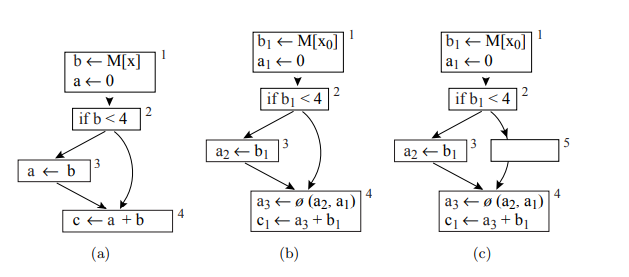
\includegraphics[width=0.8\textwidth]{p44.png}
    \caption{(a) A program with a control-flow join; (b) the program transformed to single-assignment form; (c) edge-split SSA form.}
    \label{fig:p44}
\end{figure}


unlike ordinary mathematical functions, $\Phi$(a1, a2) yields a1 if control reaches block 4 along the edge $2 \rightarrow 4$, and yields a2 if control comes in on edge $3 \rightarrow 4$.


\subsubsection{How does the $\phi$-function know which edge was taken?}


If we must execute the program, or translate it to executable form, we can “implement” the $\Phi$-function using a move instruction on each incoming edge as shown in Figure \ref{fig:p39-40}. However, in many cases, we simply need the connection of uses to definitions and don’t need to “execute” the $\Phi$-functions during optimization. In these cases, we can ignore the question of which value to produce.

\begin{figure}[htb]
     \centering
     \begin{subfigure}{0.3\textwidth}
     \centering
         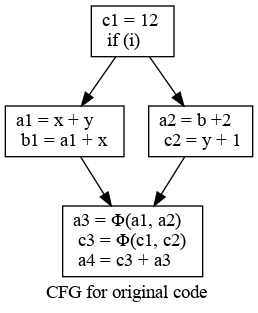
\includegraphics[width=\textwidth]{p39.png}
         \caption{Original code}
         \label{fig:p39}
     \end{subfigure}
     \begin{subfigure}{0.3\textwidth}
     \centering
         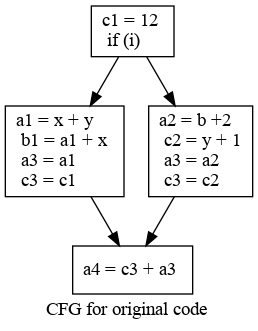
\includegraphics[width=\textwidth]{p40.png}
         \caption{Code after moving instruction.}
         \label{fig:p40}
     \end{subfigure}
        \caption{Implementing $\Phi$-function}
        \label{fig:p39-40}
\end{figure}




\subsection{Converting to SSA form}

The algorithm for converting a program to SSA form is roughly as follows:

\begin{itemize}
    \item 1. adds $\Phi$ functions for the variables, and then
    \item 2. renames all the definitions and uses of variables using subscripts.
\end{itemize}




\subsubsection{Trivial SSA}

Trivial SSA form is based on a simple observation: $\Phi$ functions are only needed for variables that are "live" after the $\Phi$ function.

\begin{itemize}
    \item Each assignment generates a fresh variable.
    \item At each join point insert $\Phi$ for all live variables.
\end{itemize}


Trivial SSA will generate some useless $\Phi$ functions. An example is shown in Figure \ref{fig:p41} So a $\Phi$-function is not needed for every variable at each point.

\begin{figure}[htb]
    \centering
    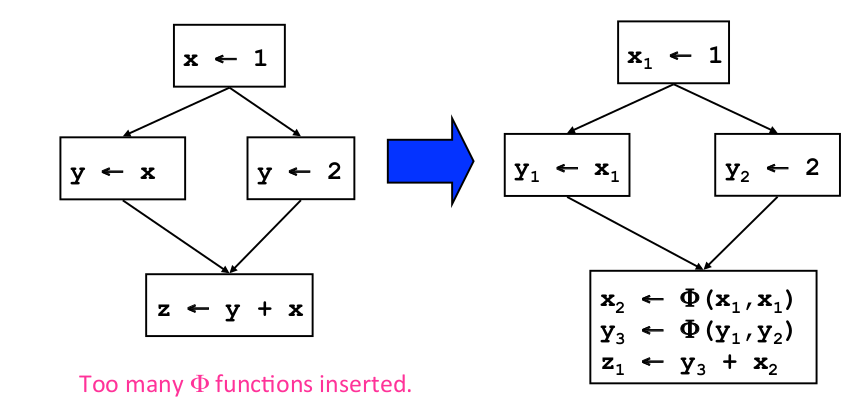
\includegraphics[width=0.5\textwidth]{p41.png}
    \caption{$x2 \leftarrow \Phi(x1,x1)$ is useless because x2 is equal to x1.}
    \label{fig:p41}

\end{figure}



\subsubsection{Minimal SSA}
Minimal SSA is an updated version compared to trivial SSA.

\begin{itemize}
    \item Each assignment generates a fresh variable.
    \item At each join point insert $\Phi$ for all live variables with multiple outstanding defs. 
\end{itemize}

\subsubsection{Path-convergence criterion}

There should be a $\Phi$-function for variable a at node z of the flow graph
exactly when all of the following are true:

\begin{itemize}
    \item 1. There is a block x containing a definition of a,
    \item 2. There is a block y (with $y \neq x$) containing a definition of a,
    \item 3. There is a nonempty path $P_{xz}$ of edges from x to z,
    \item 4. There is a nonempty path $P_{yz}$ of edges from y to z,
    \item 5. Paths $P_{xz}$ and $P_{yz}$ do not have any node in common other than z, and
    \item 6. The node z does not appear within both $P_{xz}$ and $P_{yz}$ prior to the
end, though it may appear in one or the other.
\end{itemize}


We consider the start node to contain an implicit definition of every variable, either because the variable may be a formal parameter or to represent the notion of a 
$\leftarrow$ uninitialized without special cases. A $\Phi$-function itself counts as a definition of a, so the path-convergence criterion must be considered as a set of equations to be satisfied. As usual, we can solve them by iteration as shown in \ref{alg:Iterated path-convergence criterion}.


\begin{algorithm}
\caption{Iterated path-convergence criterion}\label{alg:Iterated path-convergence criterion}
\begin{algorithmic}

\While{there are nodes $x, y, z$ satisfying conditions 1–5
and \\ $z$ does not contain a $\Phi$-function for a}
\State  insert a $\leftarrow$ $\Phi$(a, a, . . . , a) at node Z
\EndWhile
\end{algorithmic}
\end{algorithm}

\subsubsection{Dominance property of SSA form}

The iterated path-convergence algorithm for placing $\Phi$-functions is not practical, since it would be very costly to examine every triple of nodes x, y, z, and every path leading from x and y.  A much more efficient algorithm using the dominator tree of the flow graph as shown in Figure \ref{fig:p45}.


\begin{figure}[H]
    \centering
    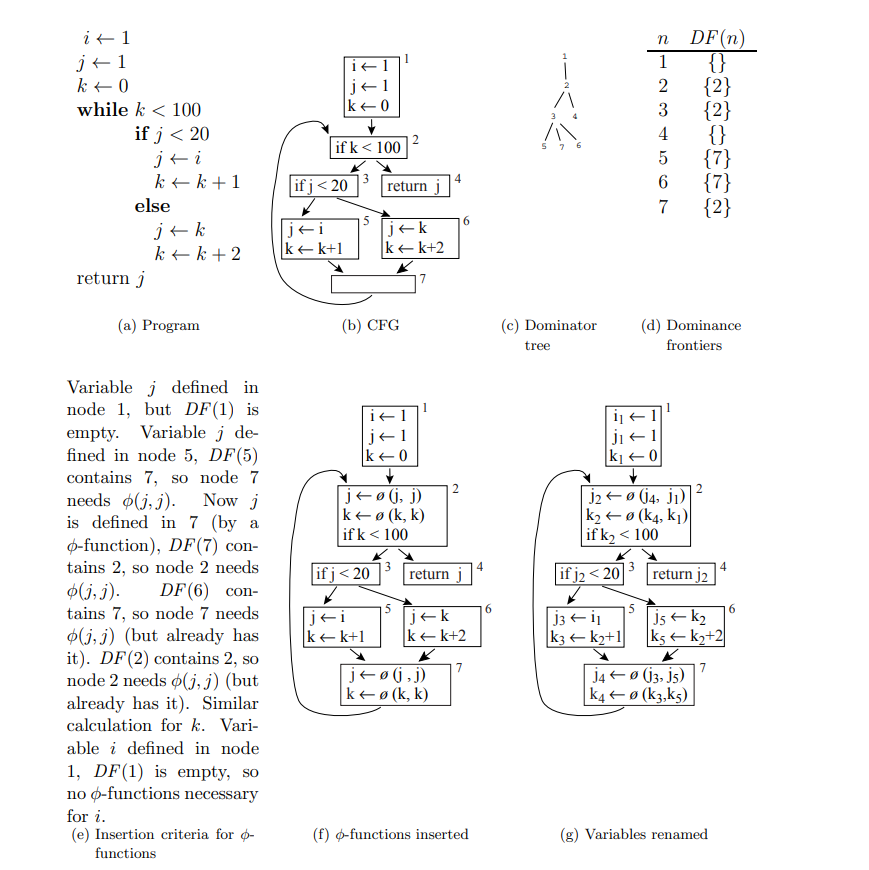
\includegraphics[width=\textwidth]{p45.png}
    \caption{ Conversion of a program to static single-assignment form. Node 7 is a postbody node, inserted to make sure there is only one loop edge; such nodes are not strictly necessary but are sometimes helpful.}
    \label{fig:p45}

\end{figure}


\begin{definition}{Strictly dominance}
    x strictly dominates w (x sdom w) iff impossible to reach w without passing through x first.
\end{definition}

\begin{definition}{Dominance}
    x  dominates w (x dom w) iff x sdom w or x = w.
$$
\operatorname{Dom}(n)= \begin{cases}\{n\} & \text { if } n=n_0 \\ \{n\} \cup\left(\bigcap_{p \in \operatorname{preds}(n)} \operatorname{Dom}(p)\right) & \text { if } n \neq n_0\end{cases}
$$
\end{definition}

\begin{definition}{Dominance tree}
    x sdom w iff x is a proper ancestor of w.  

\end{definition}

\begin{definition}{Dominance Frontier}


The dominance frontier of a node x is the set of all nodes w such that
x dominates a predecessor of w, but does not strictly dominate w.

$$
F(x)=  \{w | \texttt{x  dom pred(w) AND   !(x  sdom  w) } \}
$$
\end{definition}





An essential property of static single assignment form is that definitions dominate uses; more specifically,
\begin{itemize}
    \item  If x is the ith argument of a $\Phi$-function in block n, then the definition of x dominates the ith predecessor of n.
    \item  If x is used in a non-$\Phi$ statement in block n, then the definition of x dominates n
\end{itemize}

\begin{note}{Dominance Property of SSA	}
  In SSA,

  \begin{itemize}
      \item If x i is used in $x \leftarrow \Phi (..., x_i , ...)$, then $BB(x_i )$ dominates ith predecessor of $BB(\Phi)$
      \item If x is used in $y \leftarrow ...x...$,then BB(x) dominates BB(y)
  \end{itemize}
\end{note}


\textbf{ \large \textit{Dominance frontier criterion.}} Whenever node x contains a definition of some variable a, then any node z in the dominance frontier of x needs a $\Phi$-function for a.


\textbf{ \large \textit{Iterated dominance frontier.}} Since a $\Phi$-function itself is a kind of definition, we must iterate the dominance-frontier criterion until there are no nodes that need $\Phi$-functions.


\textbf{ \large \textit{Theorem.}} The iterated dominance frontier criterion and the iterated path convergence criterion specify exactly the same set of nodes at which to put $\Phi$-functions

\begin{figure}[htb]
    \centering
    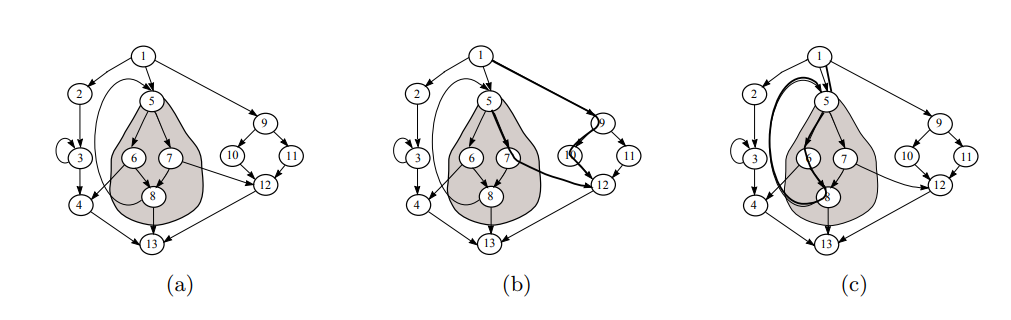
\includegraphics[width=\textwidth]{p46.png}
    \caption{Node 5 dominates all the nodes in the grey area. (a) Dominance frontier of node 5 includes the nodes (4, 5, 12, 13) that are targets of edges crossing from the region dominated by 5 (grey area including node 5) to the region not strictly dominated by 5 (white area including node 5). (b) Any node in the dominance frontier of n is also a point of convergence of nonintersecting paths, one from n and one from the root node. (c) Another example of converging paths $P_{1,5}$ and $P_{5,5}$.}
    \label{fig:p46}

\end{figure}


\begin{proof}{Proof}
The sketch of a proof that shows if w is in the dominance frontier of a definition, then it must be a point of convergence.

Suppose there is a definition of variable a at some node n (such as node 5 in Figure  \ref{fig:p46}b), and node w (such as node 12 in Figure  \ref{fig:p46}b) is in the dominance frontier of n. The root node implicitly contains a definition of every variable, including a. There is a path $P_{rw}$ from the root node (node 1 in Figure \ref{fig:p46}) to w that does not go through n or through any node that n dominates; and there is a path $P_{nw}$ from n to w that goes only through dominated nodes. These paths have w as their first point of convergence.
\end{proof}


\subsection{Computing the dominance frontier}

To insert all the necessary $\Phi$-functions, for every node n in the flow graph we need DF[n], its dominance frontier. Given the dominator tree, we can efficiently compute the dominance frontiers of all the nodes of the flow graph in one pass. We define two auxiliary sets

\begin{itemize}
    \item $DF_{local}[n]$ The successors of n that are not strictly dominated by n;
    \item $DF_{up}[n]$ Nodes in the dominance frontier of n that are not dominated by n’s immediate dominator.
\end{itemize}

The dominance frontier of n can be computed from $DF_{local}[n]$  and $DF_{up}[n]$ 


$$
D F[n]=D F_{\text {local }}[n] \quad \cup \quad \bigcup_{c \in \text { children }[n]} D F_{\text {up }}[c]
$$

where children[n] are the nodes whose immediate dominator (idom) is n.


To compute $DF_{local}[n]$ \ref{alg:computeDF} more easily (using immediate dominators instead of dominators), we use the following theorem: $DF_{local}[n]$ = the set of those successors of n whose immediate dominator is not n. The following computeDF function should be called on the root of the dominator tree (the start node of the flow graph). It walks the tree computing DF[n] for every node n: it computes $DF_{local}[n]$ by examining the successors of n, then combines $DF_{local}[n]$ and (for each child c) $DF_{up}[n]$.a

\begin{algorithm}
\caption{computeDF}\label{alg:computeDF}
\begin{algorithmic}

\State $S \gets \{\}$
\For{each node y in succ[n]} \Comment{This loop computes $DF_{local}[n]$}
\If {idom(y) $\neq$ n}
\State $S\leftarrow S \cup \{y\}$
\EndIf 
\EndFor

\For{each child c of n in the dominator tree} 
\State computeDF[c]
\For{each element w of DF[c]} \Comment{This loop computes $DF_{up}[n]$}
\If {n does not dominate w}
\State $S\leftarrow S \cup \{w\}$
\EndIf 
\EndFor
\EndFor
\end{algorithmic}
\end{algorithm}

This algorithm is quite efficient. It does work proportional to the size (number of edges) of the original graph, plus the size of the dominance frontiers it computes. Although there are pathological graphs in which most of the nodes have very large dominance frontiers, in most cases the total size of all the DFs is approximately linear in the size of the graph, so this algorithm runs in “practically” linear time.




\subsection{Inserting $\Phi$-functions}

Starting with a program not in SSA form, we need to insert just enough $\Phi$-functions to satisfy the iterated dominance frontier criterion. To avoid re-examining nodes where no $\Phi$-function has been inserted, we use a work-list algorithm.

\begin{algorithm}
\caption{Place-$\Phi$-Functions}\label{alg:Place-Phi-Functions}
\begin{algorithmic}
\For{each node n}
\For{each variable a in $A_{orig}[n]$}
\State defsites[a] $\gets$ defsites[a] $\cup \{n\}$
\EndFor
\EndFor


\For{each variable a}
\State W $\gets$ defsites[a]
\While{ W not empty}
\State{remove some node n from W}
\For{each y in DF[n]}
\If{y $\not\in$ $A_{\Phi}[a]$}
\State{insert the statement a $\gets$ $\Phi$(a, a, . . . , a) at the top of block y, where the $\Phi$-function has as many arguments as y has predecessors}
\State{$A_{\Phi}[a] \gets A_{\Phi}[a] \cup \{ y\}$}
\If{a $\not\in$ $A_{orig}[y]$}
\State{$W \gets W \cup \{y \}$}
\EndIf

\EndIf
\EndFor
\EndWhile
\EndFor

\end{algorithmic}
\end{algorithm}


Algorithm\ref{alg:Place-Phi-Functions} starts with a set V of variables, a graph G of controlflow nodes – each node is a basic block of statements – and for each node n a set $A_{orig}$[n] of variables defined in node n. The algorithm
computes $A_{\Phi}[a]$, the set of nodes that must have $\Phi$-functions for variable
a. Sometimes a node may contain both an ordinary definition and a
$\Phi$-function for the same variable; for example, in Figure \ref{fig:p46}b, a $\in$ $A_{orig}[2]$
and 2 $\in$ $A_{\Phi}[a]$.


This algorithm does a constant amount of work (a) for each node and edge in the control-flow graph, (b) for each statement in the program, (c) for each element of every dominance frontier, and (d) for each inserted $\Phi$-function. For a program of size N, the amounts a and b are proportional to N, c is usually approximately linear in N. The number of inserted $\Phi$-functions (d) could be $N^2$ in the worst case, but empirical measurement has shown that it is usually proportional to N. So in practice, Algorithm \ref{alg:Place-Phi-Functions} runs in approximately linear time.


\subsection{Renaming the variables}

After the $\Phi$-functions are placed, we can walk the dominator tree, renaming the different definitions (including $\Phi$-functions) of variable a to a1, a2, a3 and so on. Rename each use of a to use the closest definition d of a that is above a in the dominator tree. Algorithm  renames all uses and definitions of variables, after the $\Phi$-functions have been inserted by Algorithm \ref{alg:Renaming variables}. In traversing the dominator tree, the algorithm “remembers” for each variable the most recently defined version of each variable, on a separate stack for each variable. Although the algorithm follows the structure of the dominator tree – not the flow graph – at each node in the tree it examines all outgoing flow edges, to see if there are any $\Phi$-functions whose operands need to be properly numbered.



\begin{algorithm}
\caption{Renaming variables.}\label{alg:Renaming variables}
\begin{algorithmic}
\State Initialization:

\For{each variable a}
\State{Count[a] $\gets$ 0}
\State{Stack[a] $\gets$ empty}
\State{push 0 onto Stack[a]}
\EndFor

\State{Rename(n) }
\For{each statement S in block n}
\If{S is not a $\Phi$-function}
\For{each use of some variable x in S}
\State{i $\gets$ top(Stack[x])}
\State{replace the use of x with $x_i$ in S}
\EndFor
\EndIf
\For{each definition of some variable a in S}

\State Count[a] $\gets$ Count[a]+1
\State i $\gets$ Count[a]
\State push i onto Stack[a]
\State replace definition of a with definition of $a_i$ in S
\EndFor
\EndFor

\For{each successor Y of block n,}
\State Suppose n is the jth predecessor of Y
\For{each $\Phi$-function in Y}
\State suppose the jth operand of the $\Phi$-function is a
\State i $\gets$ top(Stack[a])
\State replace the jth operand with $a_i$

\EndFor
\EndFor
\For{each child X of n}
\State Rename(X)
\EndFor
\For{each definition of some variable a in the original S}
\State pop Stack[a]
\EndFor
\end{algorithmic}
\end{algorithm}




\subsection{Edge Splitting}

Some analyses and transformations including reverse transformation from SSA back into a normal form are simpler if there is never a controlflow edge that leads from a node with multiple successors to a node with multiple predecessors. To give the graph this unique successor or predecessor property, we perform the following transformation: For each control-flow edge a $\gets$ b such that a has more than one successor and b has more than one predecessor, we create a new, empty controlflow node z, and replace the a $\gets$ b edge with an a $\gets$ z edge and a z $\gets$ b edge.

An SSA graph with this property is in edge-split SSA form. Figure \ref{fig:p44} illustrates edge splitting. Edge splitting may be done before or after insertion of $\Phi$-functions.